\chapter{Paths in Graphs}
\label{chapter:paths}
\section{Connectivity}
Imagine you are developing a game, where the map is generated automatically.
In this gate there are several areas connected by portals. So you need to check
that all the areas in your map are reachable from one another.

First we need to somehow understand what we mean by ``reachable'', we say that
an area $A$ is reachable from an area $B$ if there is a path from $A$ to
$B$. To formalize this notion using graphs we need to introduce a graph
corresponding to the map, consider a graph $G = (V, E)$ such that vertices of
the graph are areas in your map and $(A, B) \in E$ iff the areas $A$ and $B$
are connected by a portal. So a path from $A$ to $B$ is a sequence of areas
$A = C_1$, \dots, $C_\ell = B$ such that $C_i$ and $C_{i + 1}$ are connected by
a portal (i.e. $(C_i, C_{i + 1}) \in E$).
\begin{definition}
  Let $G = (V, E)$ be a graph. We say that a path from $u$ to $v$ is
  a sequence $w_1, \dots, w_\ell \in V$\footnote{%
    Usually such an object is called a walk, and it is called a path if
    all the vertices $w_1$, \dots, $w_\ell$ are different. However,
    for our applications it does not matter and we will use the word ``path''.
  } such that
  \begin{itemize}
    \item $w_1 = u$, $w_\ell = v$, and
    \item $(w_i, w_{i + 1}) \in E$ for $i \in [\ell - 1]$.
  \end{itemize}

  We say that $u, v \in V$ are connected iff there is a path from $u$ to $v$.
  So the graph is connected iff any $u, v \in V$ are connected.
\end{definition}

\begin{exercise}
  Let $G = ([2n], E)$ be a graph such that $(i, j) \in E$ if $|i - j| = 2$.
  Is $G$ connected?
\end{exercise}

So, using this notation, we need to check whether the graph corresponding to
the map is connected. There are numerous ways to do it, we consider a simple
algorithm just to see how it works.
\begin{algorithm}
  \begin{algorithmic}[1]
    \Function{Connected}{$n$, $E$}
      \State $S \gets \emptyset$
      \State $Q \gets \set{1}$

      \label{algorithm:connectivity-cycle}
      \While{$Q \neq \emptyset$}
        \State Choose an element $v$ from $Q$
        \State $Q \gets S \setminus \set{v}$

        \State $S \gets S \cup \set{v}$

        \State $Q \gets Q \cup
          \set[{(v, u) \in E \text{ and } u \notin S}]{u \in \range{n}}$
      \EndWhile
      \label{line:connectivity-last}
      \State \Return{$S = \range{n}$}
    \EndFunction
  \end{algorithmic}
  \caption{An algorithm checking whether the graph on $[n]$ with the set of
  edges $E$ is connected.}
  \label{algorithm:connectivity}
\end{algorithm}

\begin{theorem}
  Algorithm~\ref{algorithm:connectivity} checks whether the graph $([n], E)$
  is connected.
\end{theorem}
\begin{proof}
  First of all, note that the algorithm has a finite running time since
  size of $S$ increases by $1$ in the cycle starting on
  line~\ref{algorithm:connectivity-cycle}.
  It is also easy to see that if a vertex $v \in Q$ at some point it is
  in $S$ on line~\ref{line:connectivity-last}. In addition, if $v \in Q$
  at some point, then $\set[{(v, u) \in E}]{u \in \range{n}} \subseteq S$ on
  line~\ref{line:connectivity-last}.

  Therefore if $u \notin S$ and $(v, u) \in E$,
  then $v \notin S$. Using this observation we may prove that
  if $G = ([n], E)$ is connected, then Algorithm~\ref{algorithm:connectivity}
  returns true. Indeed, assume the opposite. Consider $u \in \range{n} \setminus S$,
  and $N_i \subseteq \range{n}$ such that \[
    N_0 = \set{u},
    N_{i + 1} = N_i \cup \set[{w \in N_i, (v, w) \in E}]{v \in \range{n}}.
  \]
  Note that by the previous observation if $v \in N_i$, then $v \notin S$.
  Since $G$ is connected, there is a path $u = v_1, \dots, v_k = 1$.
  Note that $u \in N_0$, $v_2 \in N_1$, \dots, $v_k \in N_{k - 1}$.
  Therefore $1 = v_k \notin S$ which is a contradiction.

  To finish the proof we need to show that if $S = \range{n}$, then the graph is
  connected. To prove the statement we prove by induction that there is a path
  from $1$ to any element of $S$ and $Q$ in every iteration of
  line~\ref{algorithm:connectivity-cycle}. Indeed, initially $S$ is empty and
  $Q$ contains only $1$. After an iteration of
  line~\ref{algorithm:connectivity-cycle} we choose an element $v$ from $Q$
  and by the induction hypothesis there is a path from $1$ to $v$.
  We add it to $S$ and the statement about $S$ holds, afterwards we
  add all the neighbours of $v$ to $Q$. So the statement about $Q$ is
  also true.
\end{proof}

Not all the graphs are connected, but it is always possible to split the
graph into connected parts, such parts are called connected components.
\begin{definition}
  Let $G = (V, E)$ be a graph. We say that $U \subseteq V$ is a connected
  component if for any $u \in U$ and $v \in V$,
  $v \in U$ iff there is a path from $u$ to $v$ in $G$.
\end{definition}

\begin{theorem}
  Let $G = (V, E)$ be a graph.
  If $U_1$ and $U_2$ are connected components of $G$, then they
  either equal to each other or disjoint.
  Moreover there are connected components
  $V_1$, \dots, $V_k$ in $G$ such that $V_1 \cup \dots \cup V_k = V$
  and $V_1$, \dots, $V_k$ are disjoint.
\end{theorem}

\begin{exercise}
  Let $G = ([2n], E)$ be a graph such that $(i, j) \in E$ if $|i - j| = 2$.
  Find all the connected components of $G$.
\end{exercise}

\begin{exercise}
  Find a modification of Algorithm~\ref{algorithm:connectivity}
  that can find all the connected components of $([n], E)$.
\end{exercise}

\section{Eulerian Paths}

Graph theory originated from a simple question asked by Leonard Euler:
``Is it possible to walk through the town of K\"{o}nigsberg, starting and
ending at the same place, so that we use each bridge exactly once?'' (the map of
K\"{o}nigsberg is depicted on Figure~\ref{figure:konigsberg}).
\begin{figure}
  \begin{center}
    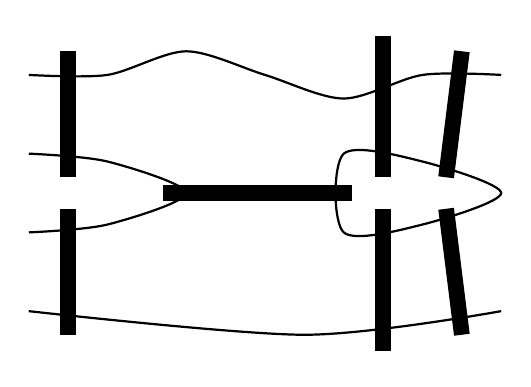
\begin{tikzpicture}[thick]
      \draw plot [smooth] coordinates {(0,0) (1, 0) (2,0.3) (3,0) (4,-0.3) (5, 0) (6, 0)};
      \draw plot [smooth] coordinates {(0, -3) (3.5, -3.3) (6, -3)};

      \draw plot [smooth] coordinates {(0,-1) (1, -1.1) (2, -1.5) (1, -1.9) (0,-2)};

      \draw plot [smooth cycle] coordinates {(4, -1) (5, -1.1) (6, -1.5) (5, -1.9) (4, -2)};

      \draw [line width=2mm] (0.5, 0.3) -- (0.5, -1.3);
      \draw [line width=2mm] (0.5, -3.3) -- (0.5, -1.7);
      \draw [line width=2mm] (4.5, 0.5) -- (4.5, -1.3);
      \draw [line width=2mm] (4.5, -3.5) -- (4.5, -1.7);
      \draw [line width=2mm] (5.5, 0.3) -- (5.3, -1.3);
      \draw [line width=2mm] (5.5, -3.3) -- (5.3, -1.7);
      \draw [line width=2mm] (1.7, -1.5) -- (4.1, -1.5);
    \end{tikzpicture}
  \end{center}
  \caption{K\"{o}nigsberg's map}
  \label{figure:konigsberg}
\end{figure}
It is possible to see that the geometry of the islands is not important for
this problem, the only important property is the number of bridges between
islands.

In other words, all the necessary information can be described by the graph
(the islands are vertices and the bridges are edges) depicted on
Figure~\ref{figure:konigsberg-graph}.
\begin{figure}
  \begin{center}
    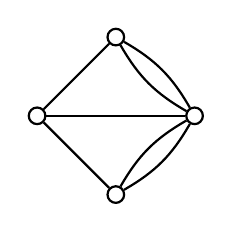
\begin{tikzpicture}[thick]
      \node[circle, draw, inner sep=0pt, minimum size=6pt] (v1) at (0,0) {};
      \node[circle, draw, inner sep=0pt, minimum size=6pt] (v2) at (1,1) {};
      \node[circle, draw, inner sep=0pt, minimum size=6pt] (v3) at (-1,1) {};
      \node[circle, draw, inner sep=0pt, minimum size=6pt] (v4) at (0,2) {};

      \draw (v4) to[out=-60, in=150] (v2);
      \draw (v4) to[out=-30, in=120] (v2);
      \draw (v1) to[out=60, in=-150] (v2);
      \draw (v1) to[out=30, in=-120] (v2);
      \draw (v2) -- (v3);
      \draw (v1) -- (v3);
      \draw (v4) -- (v3);
    \end{tikzpicture}
  \end{center}
  \caption{The graph of K\"{o}nigsberg's bridges}
  \label{figure:konigsberg-graph}
\end{figure}
Hence, to formalize the problem we need to give the following definition.
\begin{definition}
  A path $v_1$, \dots, $v_k$ in a graph $G = (V, E)$ is called Eulerian if for
  any edge $(u_1, u_2) \in E$ there is exactly one $i \in [k - 1]$ such that
  $u_1 = v_i$ and $u_2 = v_{i + 1}$.

  An Eulerian path is called an Eulerian cycle if $v_1 = v_k$.
\end{definition}
Using this definition the question is whether there exists an Eulerian cycle in
the graph of K\"{o}nigsberg's bridges.

\begin{exercise}
  Check whether the graph of K\"{o}nigsberg's bridges has an Eulerian cycle or
  not.
\end{exercise}

The following theorem gives a simple criterion that allows us to solve the
problem in the general case.
\begin{theorem}
\label{theorem:eulerian}
  A connected graph $G$ has an Eulerian cycle if and only if all vertices
  of $G$ have even degree.
  (Note that the statement holds even if $G$ has parallel edges).
\end{theorem}

\begin{proof}
  Assume that such a cycle exists
  If a vertex $v$ appears $k$ times in the cycle, then there are $2k$ edges
  involving $v$ in the cycle (because, each time $v$ is visited, there is an
  edge used to step on $v$ and one to leave from $v$); since the cycle contains
  all the edges of the graph, $v$ has degree $2k$. Therefore all vertices have
  even degree. This shows that if a connected graph contains an Eulerian cycle,
  then every vertex has even degree.

  To prove this statement in the other direction, we will prove by induction a
  stronger statement, we will prove that if $G$ is a graph in which every
  vertex has even degree, then every connected non-trivial connected
  component of $G$ (a connected component is trivial if it contains only an
  isolated vertex of degree zero) has an Eulerian cycle. We will proceed by
  induction on the number of edges.

  If there are zero edges, then every connected component has only one vertex
  and so it is nothing to prove. This is the base case of the induction.

  If we have a graph $G = (V,E)$ with a non-empty set of edges and in which
  every vertex has even degree, then let $V_1$, \dots, $V_m$ be the non-trivial
  connected components of $V$. If $m \ge 2$, then every connected component has
  strictly less vertices than $G$, and so we can apply the inductive hypothesis
  and find Eulerian cycles in each of $V_1$, \dots, $V_m$.

  It remains to consider the case in which the set $V'$ of vertices of non-zero
  degree of $G$ are all in the same connected component. Let $G' = G[V']$.
  Since every vertex of $G'$ has degree at least, there must be a cycle in
  $G'$. Let $C$ be a simple cycle (that is, a cycle with no vertices repeated)
  in $G'$, and let $G'' - C$. Since we have removed two edges from every
  vertex, we have that $G''$ is still a graph in which every vertex has even
  degree. Since $G''$ has fewer edges than $G'$ we can apply the induction
  hypothesis, and find an Eulerian cycle in each non-trivial connected
  component of $G''$. We can then patch together these Eulerian cycles with $C$
  as follows: we traverse $C$, starting from any vertex; the first time we
  reach one of the non-trivial connected components of $G''$, we stop
  traversing $C$, and we traverse the Eulerian cycle of the component, then
  continue on $C$, until we reach for the first time one of the non-trivial
  connected components of $G''$ that we haven’t traversed yet, and so on. This
  describes a Eulerian path into all of $G'$
\end{proof}

\begin{exercise}
  Finish the proof of Theorem~\ref{theorem:eulerian} by proving that if a graph
  $G$ has only vertices of an odd degree, then there is a simple cycle in $G$.
\end{exercise}

\begin{corollary}
  A graph $G$ has an Eulerian path starting and ending in two different
  vertices if and only if in $G$ there are exactly two vertices with odd
  degrees.
  (Note that the statement holds even if $G$ has parallel edges).
\end{corollary}
\begin{proof}
  Let $G = (V, E)$ and $u$ and $v$ be the vertices with odd degrees. Let us
  consider the graph $G + (u, v) = (V, E \cup (u, v))$ (if there are edges
  between $u$ and $v$ we increase their number by one). Note that all
  the degrees in $G + (u, v)$ are even.
  \nomenclature[G]{$G + e$}{denotes the graph $(V, E \cup \set{e})$}
  Therefore by Theorem~\ref{theorem:eulerian}, there is an Eulerian cycle in
  $G + (u, v)$. Without loss of generality the cycle is in the form $u$, $v$,
  $w_1$, \dots, $w_k$, $v$. Therefore, there is an Eulerian path $v$,
  $w_1$, \dots, $w_k$, $v$ in $G$.
\end{proof}

\section{Hamiltonian Paths}

Another example of a path that mathematicians are interested in is Hamiltonian
path.
\begin{definition}
  Let $G$ be a graph. We say that a path in $G$ is Hamilton
  if it visits every vertex in $G$ exactly once. We say that such a path is a
  Hamiltonian cycle if its starting and ending vertices are
  connected.\footnote{%
    Hamiltonian paths and cycles are named after William Rowan Hamilton who
    invented the icosian game, now also known as Hamilton's puzzle, which
    involves finding a Hamiltonian cycle in the edge graph of the dodecahedron.
  }
\end{definition}

The greatest difference with Eulerian cycles is that it is not known whether
there is a fast (polynomial-time) algorithm that allows to find the Hamiltonian
cycles in a graph.\footnote{%
  Proving or disproving that there is a polynomial-time algorithm allowing to
  check whether a graph $G$ has a Hamiltonian path is one of the Millennium
  Problems. Clay Mathematics Institute offers a prize of \$1 million to a person
  who solves the problem.
}

It is easy to design an algorithm that checks whether a path exists in
$O((n - 1)!)$ by just brute forcing all the possible candidates for such a path.
However, using the ideas of the inclusion-exclusion principle, we may design
a much faster algorithm.
\begin{theorem}
\label{theorem:hamiltonian-algorithm}
  There is an algorithm with the running time $O(2^n n^3)$ such that it finds
  the number of Hamiltonian cycles in a graph $G = ([n], E)$.
\end{theorem}

Before we prove the theorem, recall that if $U$ and
$A_1, \dots, A_n \subseteq U$ are some finite sets, then
\[
  \left| \bigcap_{i = 1}^n A_i \right| =
  \sum_{X \subseteq \range{n}} (-1)^{|X|}
    \left| \bigcap_{i \in X} \overline{A}_i \right|,
\]
where $\overline{A}_i = U \setminus A_i$ and
$\bigcap_{i \in \emptyset} \overline{A}_i = U$.

\begin{proof}[Proof of Theorem~\ref{theorem:hamiltonian-algorithm}]
  As we mentioned before we the inclusion-exclusion principle to find the number
  of Hamilton cycles. Let $U$ be the set of all the cycles of length $n$
  (length is the number of edges in the path) going
  via the vertex $1$ and $A_v \subseteq U$ ($v \in \range{n})$ be the set of cycles of
  length $n$ going via the vertices $1$ and $v$.

  It is clear that the answer is $\left| \bigcap_{i = 1}^n A_i \right|$.
  Therefore it is enough to find all the cardinalities of
  $\left| \bigcap_{i \in X} \overline{A}_i \right|$. Note that
  $\bigcap_{i \in X} \overline{A}_i$ is equal to the set of all the cycles of
  length $n$ going via the vertex $1$ in $G - X$. We denote the cardinality of
  this set by $C_X$.

  To find the value of $C_X$ we use the following notation.
  Let $E_X$ be the set of edges in $G - X$ and let $T_X(d, x)$ be
  the number of length $d$ paths from $1$ to $x \in \range{n} \setminus X$ in $G - X$.
  Clearly $T_X(0, x) = 1$ if $x = 1$ and $T_X(0, x) = 0$ otherwise. In addition,
  $T_X(d + 1, x) = \sum_{y ~:~ (y, x) \in E_X} T_X(d, y)$. Therefore, we may
  compute $T_X(n, x)$ for all $x \in \range{n} \setminus X$ in $n^3$ steps. As a
  result, we may find the value of $\sum_{X \subseteq \range{n}} (-1)^{|X|} C_X$ in
  $2^n n^3$ steps.
\end{proof}

However, one may prove that if all the vertices in a graph have large degree,
then the graph has a Hamiltonian cycle.
\begin{theorem}[Dirac]
  Let $G$ be a graph on $n \ge 3$ vertices. If every vertex $v$ in $G$ has
  degree at least $n / 2$, then there is a Hamiltonian cycle in $G$.
\end{theorem}
\begin{proof}
  For the sake of contradiction, let us assume that $G$ has no Hamiltonian
  cycle but all the vertices have degree at least degree $n / 2$, where $n$ is
  the number of vertices in $G$.

  Let us start adding edges to $G$ as long as we are not creating a
  Hamiltonian cycle. When we stop we get a graph $H = (V, E)$ such that
  all the vertices of $H$ have degree at least $n / 2$, $H$ does
  not have a Hamiltonian cycle, but adding any new edge would create a
  Hamiltonian cycle.

  Consider any two vertices $x$ and $y$ that are not connected by
  an edge. We know that in the graph $H + (x, y)$ there is
  a Hamiltonian cycle $x = v_1$, \dots, $v_n = y$. Note that
  $|\set[{(x, v) \in E \text{ or } (y, v) \in E}]{v \in V}| \ge n$
  since $\deg_H(x) \ge n / 2$ and $\deg_H(y) \ge n / 2$.
  Therefore by the pigeonhole principle, there is $2 \le i \le n - 1$
  such that $(x, v_i) \in E$ and $(v_{i - 1}, y) \in E$. As a result,
  $x$, $v_2$, \dots, $v_{i - 1}$, $y$, $v_{n - 1}$, \dots, $v_i$
  is a Hamiltonian cycle in $H$.
\end{proof}

There are plenty of different applications of Hamiltonian paths. Here we describe
the one that comes from bioinformatics.

Imagine that we want to read a DNA strand, i.e., determine the order in which
nucleotides occur on a strand of DNA. One of the methods, called
``Sequencing by Hybridization'', is based on Hamiltonian paths.

The method works as follows.
\begin{itemize}
  \item Attach all possible DNA probes of length $k$ to a flat surface, each
    probe at a distinct and known location. This set of probes is called
    the DNA microarray.
  \item Apply a solution containing fluorescently labeled copies of a DNA
    fragment to the array.
  \item The DNA fragment hybridizes with those probes that are
    complementary to substrings of length $k$ of the fragment.
  \item Using a spectroscopic detector, determine which probes hybridize to
    the DNA fragment to obtain the $k$-mer composition of the DNA fragment.
  \item Reconstruct the sequence of the DNA fragment from the $k$-mer
    composition.
\end{itemize}

In other words, we need to reconstruct a string $s$ from all $n - k + 1$
substrings of length $k$; e.g, we need to reconstruct the string TATGGTGC
from the strings ATG, GGT, GTG, TAT, TGC, TGG (in this example $k = 3$).
(Note that different strings may have the same sets of substrings.
Strings GTATCT and GTCTAT correspond to the strings
AT, CT, GT, TA, TC when $k = 2$.)

By a given set $p_1$, \dots, $p_\ell$ of strings ($k$-mers) of length $k$
we construct the following graph. There are $\ell$ vertices corresponding to
the strings $p_1$, \dots, $p_\ell$; there is an edge between $p_i$ and $p_j$
whenever the same string of length $k - 1$ is a suffix of $p_i$ and a
prefix of $p_j$ (for example, TG is a suffix of ATG and a prefix of TGG).
It is easy to see that we can find a string corresponding to
$p_1$, \dots, $p_\ell$ if we have a Hamiltonian path in the graph.

\begin{chapterendexercises}
  \exercise Is it true that if a graph has a closed Eulerian walk, then it has
    an even number of edges?
  \exercise[recommended] Let $G$ be a graph such that there are only $2$
    vertices with odd degree. Prove that they belong to the same connected
    component.
  \exercise Let $G = (V, E)$ be a connected graph and $c : V \to \set{0, 1}$
    be a function.
    \begin{enumerate}
      \item Assume that $\sum_{v \in V} c(v)$ is odd.
        Show that for any $s : E \to \set{0, 1}$, there is a vertex
        $v \in V$ such that $\sum_{(u, v) \in E} s(u, v)$ and $c(v)$
        have different reminders modulo $2$.
      \item Assume that $\sum_{v \in V} c(v)$ is even.
        Show that there is a function $s : E \to \set{0, 1}$
        such that $\sum_{(u, v) \in E} s(u, v)$ is odd iff $c(v)$ is odd
        for all $v \in V$.
    \end{enumerate}
  \exercise What is the maximal number of edges of a simple graph $G$ on $[n]$
    if it is not connected?
\end{chapterendexercises}
